\documentclass[13pt]{beamer}
%
% Choose how your presentation looks.
%
% For more themes, color themes and font themes, see:
% http://deic.uab.es/~iblanes/beamer_gallery/index_by_theme.html
%
\mode<presentation>
{
\usetheme{CambridgeUS}     % or try Darmstadt, Madrid, Warsaw, ...
\usecolortheme{beaver} % or try albatross, beaver, crane, ...
\usefonttheme{default}  % or try serif, structurebold, ...
\setbeamertemplate{navigation symbols}{}
\setbeamertemplate{caption}[numbered]
} 

\usepackage[english]{babel}
\usepackage[utf8x]{inputenc}
\usepackage{xcolor}
\usepackage{multicol}
\usepackage{tikz}
\usepackage{tikz-uml}
\tikzumlset{font=\footnotesize\ttfamily}
\usepackage{hyperref}

\usepackage{listings}
\definecolor{codegreen}{rgb}{0,0.6,0}
\definecolor{codegray}{rgb}{0.5,0.5,0.5}
\definecolor{codepurple}{rgb}{0.58,0,0.82}
\definecolor{backcolour}{rgb}{0.95,0.95,0.92}

\lstdefinestyle{myCustomCppStyle}{
language=C++,
numbers=left,
stepnumber=1,
numbersep=9pt,
tabsize=2,
showspaces=false,
showstringspaces=false
}

\lstset{basicstyle=\tiny,style=myCustomCppStyle}

\lstdefinestyle{mystyle}{
backgroundcolor=\color{backcolour},   
commentstyle=\color{codegreen},
keywordstyle=\color{magenta},
numberstyle=\tiny\color{codegray},
stringstyle=\color{codepurple},
basicstyle=\ttfamily\footnotesize,
breakatwhitespace=false,         
breaklines=true,                 
captionpos=b,                    
keepspaces=true,                 
numbers=left,                    
numbersep=5pt,                  
showspaces=false,                
showstringspaces=false,
showtabs=false,                  
tabsize=1
}

\lstset{style=mystyle}

\usepackage{graphicx}
\graphicspath{ {./images/} }

\usepackage{tikz}
\usetikzlibrary{decorations.text}
\usetikzlibrary{shapes.geometric, arrows, positioning, calc, matrix}

\tikzset{
basic box/.style={
shape=rectangle, rounded corners, align=center,
draw=#1, fill=#1!25},
header node/.style={
Minimum Width=header nodes,
font=\strut\Large\ttfamily,
text depth=+0pt,
fill=white, draw},
header/.style={
inner ysep=+1.5em,
append after command={
\pgfextra{\let\TikZlastnode\tikzlastnode}
node [header node] (header-\TikZlastnode) at (\TikZlastnode.north) {#1}
node [span=(\TikZlastnode)(header-\TikZlastnode)] at (fit bounding box) (h-\TikZlastnode) {}
}
},
hv/.style={to path={-|(\tikztotarget)\tikztonodes}},
vh/.style={to path={|-(\tikztotarget)\tikztonodes}},
fat blue line/.style={ultra thick, blue}
}

\definecolor{mygray}{RGB}{208,208,208}
\definecolor{mymagenta}{RGB}{226,0,116}
\newcommand*{\mytextstyle}{\sffamily\Large\bfseries\color{black!85}}
\newcommand{\arcarrow}[3]{%
% inner radius, middle radius, outer radius, start angle,
% end angle, tip protusion angle, options, text
\pgfmathsetmacro{\rin}{1.7}
\pgfmathsetmacro{\rmid}{2.2}
\pgfmathsetmacro{\rout}{2.7}
\pgfmathsetmacro{\astart}{#1}
\pgfmathsetmacro{\aend}{#2}
\pgfmathsetmacro{\atip}{5}
\fill[mygray, very thick] (\astart+\atip:\rin)
             arc (\astart+\atip:\aend:\rin)
-- (\aend-\atip:\rmid)
-- (\aend:\rout)   arc (\aend:\astart+\atip:\rout)
-- (\astart:\rmid) -- cycle;
\path[
decoration = {
text along path,
text = {|\mytextstyle|#3},
text align = {align = center},
raise = -1.0ex
},
decorate
](\astart+\atip:\rmid) arc (\astart+\atip:\aend+\atip:\rmid);
}
\title[Design Pattern]{Structural Design Pattern}
\author{Hung Tran}
\institute{Fpt software}
\date{\today}


\begin{document}

\begin{frame}
	\titlepage
\end{frame}

\begin{frame}{Outline}
	\tableofcontents
\end{frame}

\section{Structural Pattern Overview}

\begin{frame}{Structural Pattern Overview}
	\begin{center}
		\textcolor{blue}{\textbf{How classes and objects are composed to form larger structure.}}
	\end{center}
	\begin{itemize}
		\item \textbf{Adapter}: Convert the interface of a class into another interface.
		\item \textbf{Bridge}: Decouple an abstraction from its implementation.
		\item \textbf{Composite}: Compose objects into tree structure.
		\item \textbf{Decorator}: Attach additional responsibilities to an object dynamically.
		\item \textbf{Facade}: Provide a unified interface to a set of interfaces.
		\item \textbf{Flyweight}: Use sharing to support large numbers of fine-grained objects efficiently.
		\item \textbf{Proxy}: Provide a surrogate or placeholder for another object to control access to it.
	\end{itemize}
\end{frame}

\section{Composite design pattern}

\begin{frame}{Problem Statement}
	\begin{columns}[T]
		\begin{column}{.45\textwidth}
			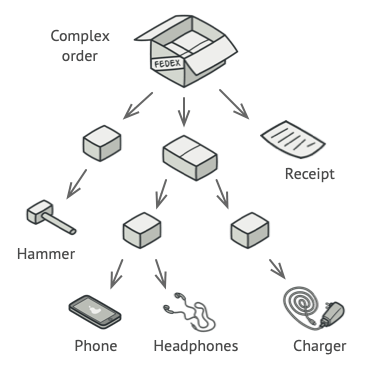
\includegraphics[scale=0.4]{./images/problem.png}
		\end{column}
	
		\begin{column}{.45\textwidth}
			\begin{itemize}
				\item Imagine that you have two types of objects: \textbf{Products} and \textbf{Boxes}
				\item A Box can contain several Products as well as a number of smaller Boxes.
				\item These little Boxes can also hold some Products or even smaller Boxes, and so on.
			\end{itemize}
		\end{column}
	\end{columns}
\end{frame}

\begin{frame}{Problem Statement}
	\begin{itemize}
		\item Create an ordering system that uses these classes
		\item Orders could contain simple products without any wrapping, as well as boxes stuffed with products...and other boxes.
		\item \textcolor{red}{How would you determine the total price of such an order?}
		\item You could try the direct approach: unwrap all the boxes, go over all the products and then calculate the total.
		\item That would be doable in the real world; but in a program, it’s not as simple as running a loop.
		\item You have to know the classes of Products and Boxes you’re going through, the nesting level of the boxes and other nasty details beforehand.
		\item All of this makes the direct approach either too awkward or even impossible.
	\end{itemize}
\end{frame}

\begin{frame}{The Intent of Composite Design Pattern}
	\begin{center}
	\textcolor{red}{\textbf{Compose objects into tree structures to represent part-whole hierarchies. Composite lets clients treat individual objects and compositions of objects uniformly.}}
	\end{center}
\end{frame}

\begin{frame}{Structure of Bridge Pattern: Object adapter}
	\begin{center}
		\begin{tikzpicture}
			\umlemptyclass[x=0,y=0]{Client}
			\umlclass[x=3,y=0]{Abstraction}{}{operation()}
			\umlclass[x=2,y=-4]{RefinedAbstruction}{}{}
			\umlclass[x=8,y=0]{Implementor}{}{operationImp()}
			\umlclass[x=6,y=-4]{ConcreteA}{}{operationImp()}
			\umlclass[x=10,y=-4]{ConcreteB}{}{operationImp()}
			\umluniaggreg{Abstraction}{Implementor}
			\umluniassoc[pos=0.95, align=right, name=uniassoc]{Client}{Abstraction}
			\umlinherit[geometry=|-|]{RefinedAbstruction}{Abstraction}
			\umlinherit[geometry=|-|]{ConcreteA}{Implementor}
			\umlinherit[geometry=|-|]{ConcreteB}{Implementor}
		\end{tikzpicture}	
	\end{center}
\end{frame}

\begin{frame}{Pointer to Implementation (PIMPL)}
	\textcolor{blue}{}
	\begin{itemize}
		\setlength\itemsep{1em}
		\item PIMPLE is the manifestation of the bridge design pattern albeit a slightly different one.
		\item PIMPL idiom is all about hiding the implementation details of a particular class by sticking it into separate implementation pointed by pointer just as the name suggests.
	\end{itemize}
\end{frame}

\begin{frame}{PIMPL implementation}
\begin{columns}[T]
\begin{column}{.45\textwidth}
\lstset{basicstyle=\tiny,style=myCustomCppStyle}
person.h
\lstinputlisting{./examples/pimpl/person.h}
\end{column}

\begin{column}{.45\textwidth}
\lstset{basicstyle=\tiny,style=myCustomCppStyle}
person.cpp
\lstinputlisting{./examples/pimpl/person.cpp}
\end{column}
\end{columns}
\end{frame}

\begin{frame}{Why would you want to do this PIMPL?}
	\textcolor{blue}{}
	\begin{itemize}
		\setlength\itemsep{1em}
		\item Security purpose: a data member which contains critical information.
		\item Compilation time
	\end{itemize}
\end{frame}

\begin{frame}{Disadvantages of PIMPL?}
	\textcolor{blue}{}
	\begin{itemize}
		\setlength\itemsep{1em}
		\item Run-time overhead as we have to dereference the pointer every time for access.
		\item Construction \& destruction overhead of unique\_ptrbecause it creates a memory in a heap
		\item We also have to bear some indirection if we want to access the data member of Person in PersonImpl like passing this pointer or so
	\end{itemize}
\end{frame}

\begin{frame}{Advantages}
	\textcolor{blue}{}
	\begin{itemize}
		\item Bridge Design Pattern provides flexibility to develop abstraction(i.e. interface) and the implementation independently. And the client/API-user code can access only the abstraction part without being concerned about the Implementation part.
		\item It preserves the Open-Closed Principle, in other words, improves extensibility as client/API-user code relies on abstraction only so implementation can modify or augmented any time.
		\item By using the Bridge Design Pattern in the form of PIMPL. We can hide the implementation details from the client as we did in PIMPL idiom example above.
		\item The Bridge Design Pattern is an application of the old advice, “prefer composition over inheritance” but in a smarter way. It comes handy when you must subclass different times in ways that are orthogonal with one another(say 2×2 problem discuss earlier).
		\item A compile-time binding between an abstraction and its implementation should be avoided. So that an implementation can select at run-time.
	\end{itemize}
\end{frame}

\begin{frame}
\begin{center}
{\fontsize{40}{50}\selectfont Thank You!}
\end{center}
\end{frame}


\end{document}
